\documentclass[11pt, oneside]{article} 
\usepackage{geometry}
\geometry{letterpaper} 
\usepackage{graphicx}
	
\usepackage{amssymb}
\usepackage{amsmath}
\usepackage{parskip}
\usepackage{color}
\usepackage{hyperref}

\graphicspath{{figures/}
                      {/Users/telliott/Desktop/figures/}
                      {/Users/telliott/Dropbox/Github-math/figures/}}
% \begin{center} \includegraphics [scale=0.4] {gauss3.png} \end{center}

\title{Excircles and Heron}
\date{}

\begin{document}
\maketitle
\Large

%[my-super-duper-separator]

\begin{center} 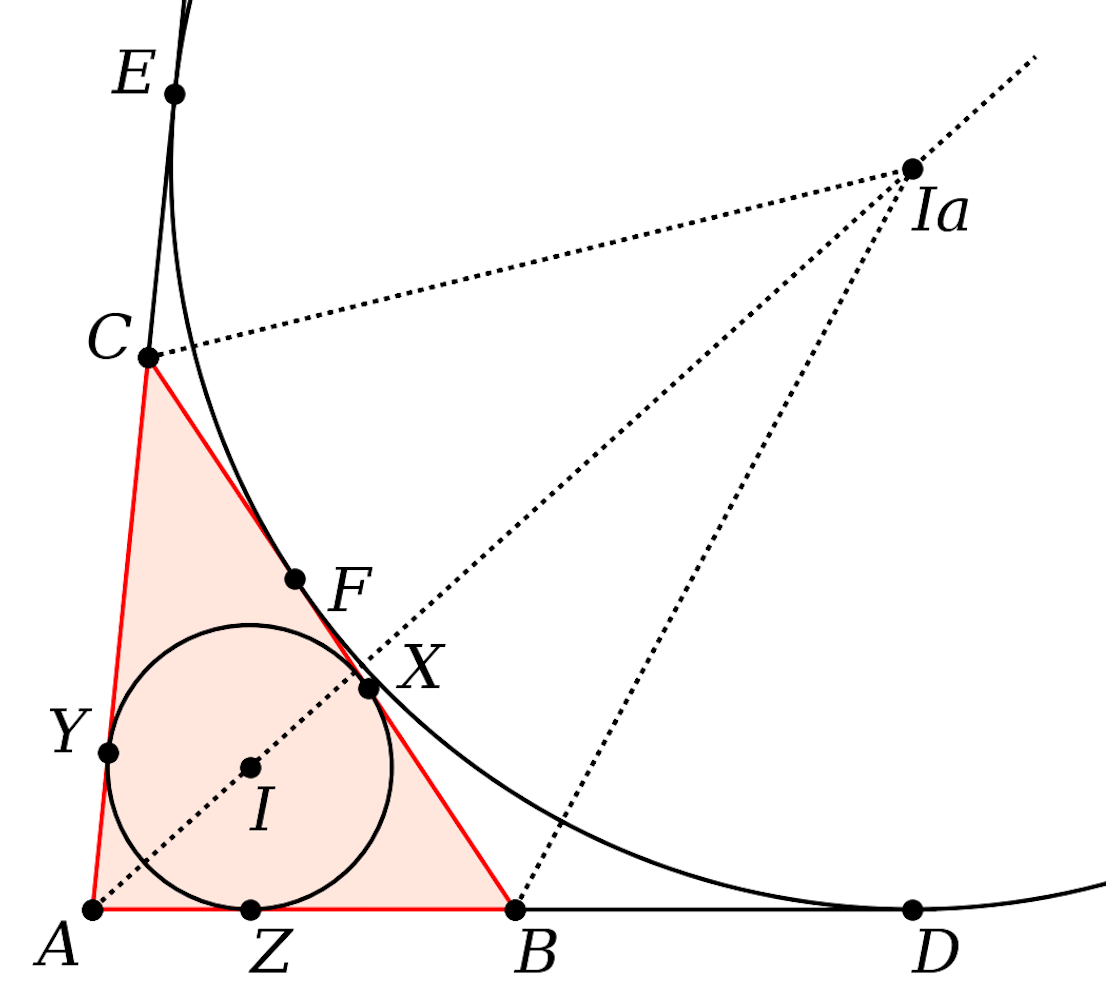
\includegraphics [scale=0.40] {excircle_crop1.png} \end{center}
Any triangle has an \emph{incircle}, defined as the circle tangent to each of the three sides of the triangle.  The incircle is on an \emph{incenter} $I$.

$I$ lies on the angle bisectors of the three angles $A$, $B$ and $C$.  The points where the incircle is tangent to the sides are marked $X$, $Y$, and $Z$, so for example $IZ \perp AB$.  The circle through $X$,$Y$ and $Z$ is tangent to each of the sides.  

\emph{Proof}.  Find $I$ as the intersection of two bisectors.  Draw pairs of right triangles such as $\triangle IZA$ and $\triangle IYA$.  These are congruent since they have two (thus three) angles the same and a shared side. So $IZ = IY = IX$.  Draw the circle through $X$, $Y$ and $Z$ on center $I$.  Since $IZ$ et al are radii, $AB \perp IZ$ is tangent to the circle at $I$.  $\square$

Each side of the triangle has a corresponding \emph{excircle}.  The excircle on center $I_a$ is the circle tangent to three lines:  side $a$ as well as the extensions of sides $AB$ and $AC$ to $D$ and $E$.

One idea for how to find the relevant points is to notice that $D$ and $E$ also tangents from $A$ to the circle we are looking for.  Hence $AD = AE$.  

So for a candidate point $D$, find $E$ the same distance from $A$ on the extension of $AC$ and then draw the perpendiculars to cross at $I_a$.  It might help a little to know that $BD + CE$ is equal in length to side $a$.  If the circle drawn on $I_a$ with radius $r = AD = AE$ is tangent to side $a$, you're done.  

\begin{center} 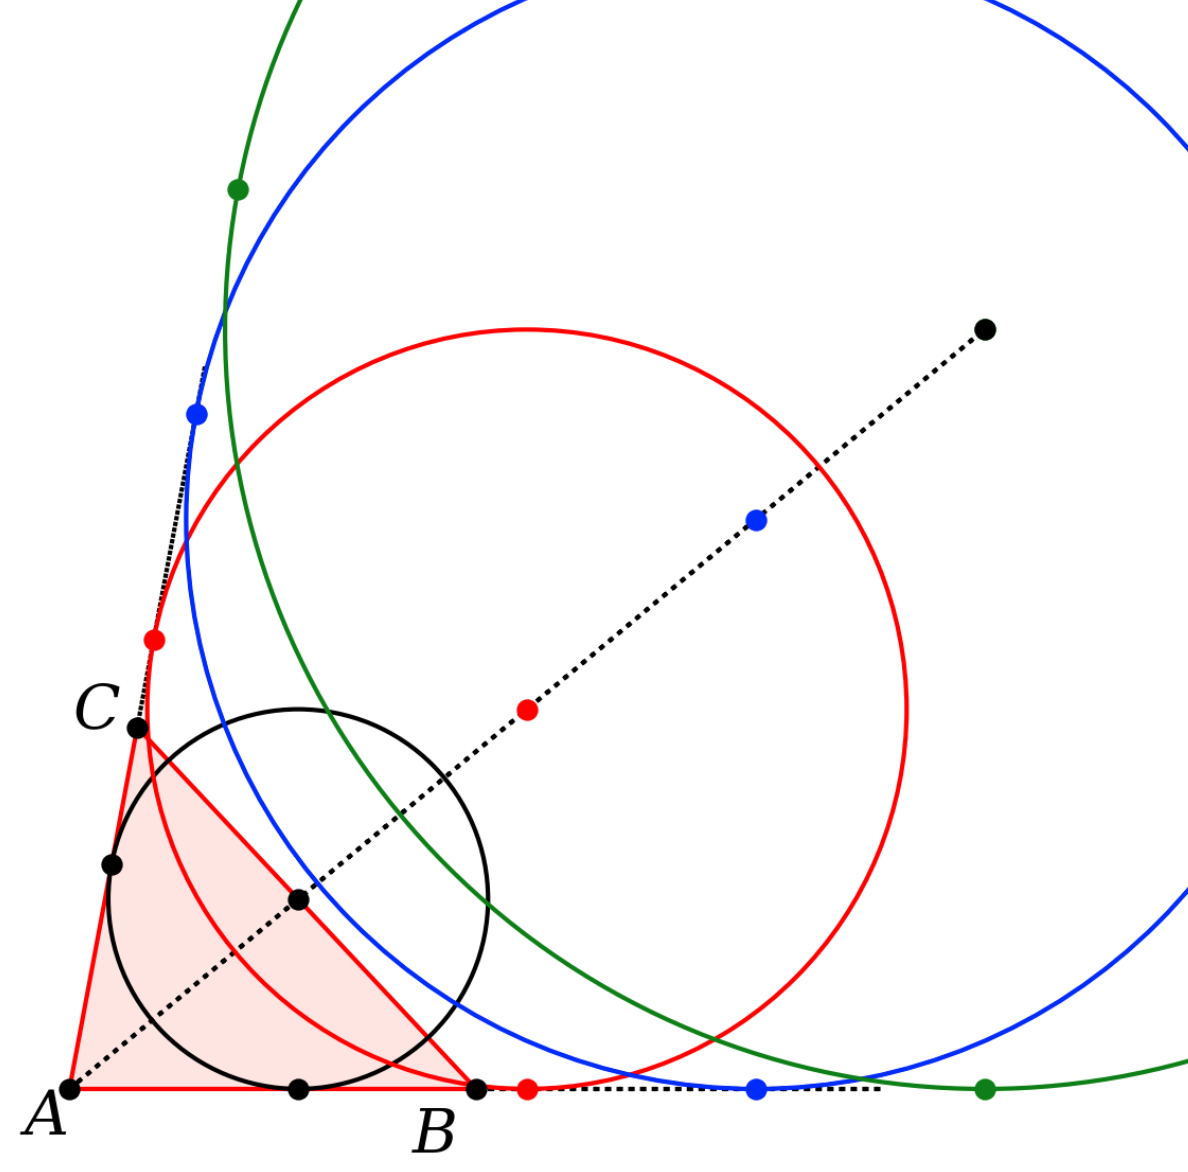
\includegraphics [scale=0.40] {excircle_crop3.png} \end{center}

In the figure above, a circle tangent to the extensions of $AB$ and $AC$ has been drawn with its center on evenly spaced points along the bisector, starting from where the bisector crosses side $a$.  The tangent points as well as the points where the circle itself crosses the bisector, are also evenly spaced.  The ratio between these distances depends only on the angle at $A$.  

The tangent point we are looking for on $BC$ does \emph{not} lie on the bisector, unless $AB = AC$ (and $\triangle ABC$ is isosceles).  Intuitively, there is one position for the center in which the circle just ``kisses'' side $a$.

More practically, $I_a$ can be found first, as the intersection of the bisectors of the external angles $\angle CBD$ and $\angle ECB$.  Then find $D$ and $E$ as points on the extensions of $AB$ and $AC$ whose perpendiculars go through $I_a$.  Last, draw the circle of radius $AD = AE$.

\begin{center} 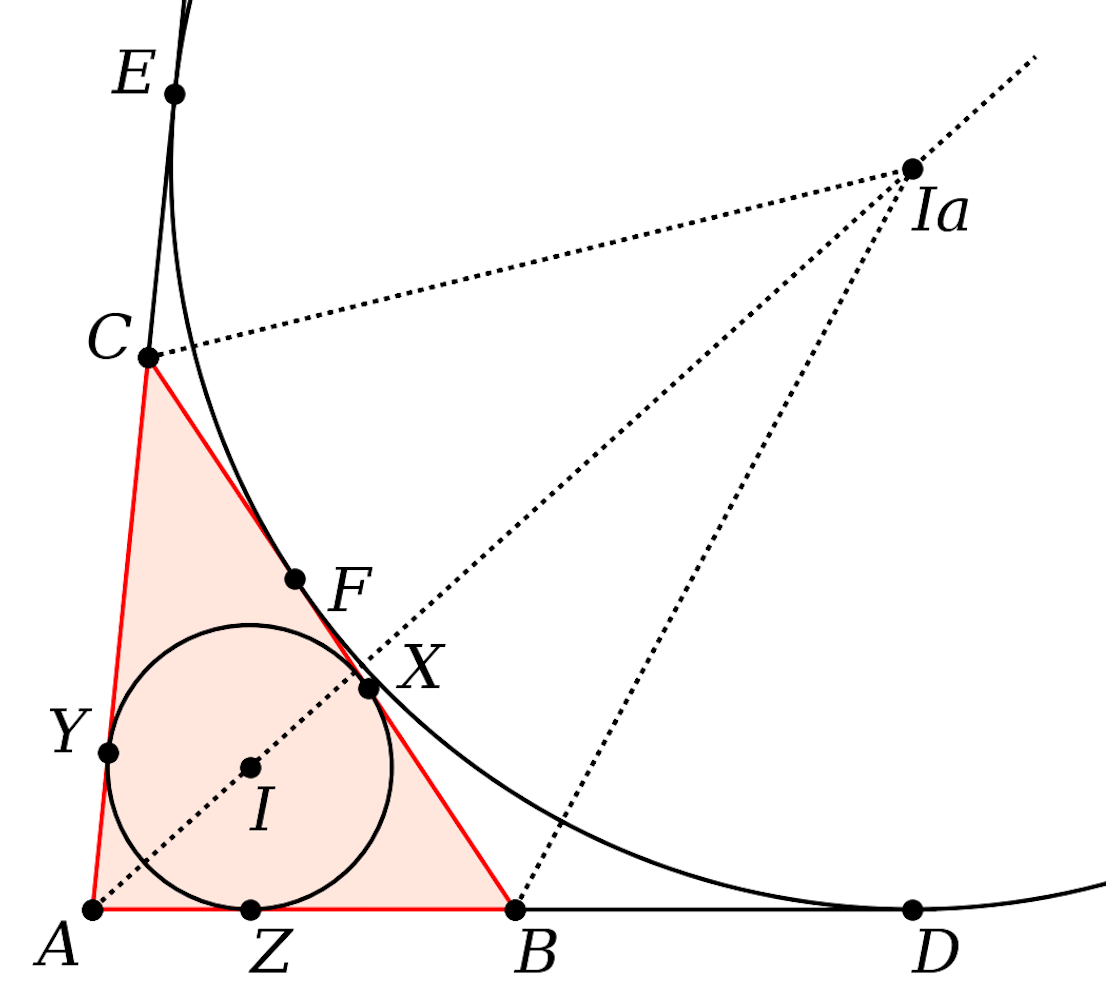
\includegraphics [scale=0.40] {excircle_crop1.png} \end{center}

We can see that this will be correct, since $BD = BF$ as tangents from $B$ and $CE = CF$ as tangents from $C$, so the bisectors of $\angle CBF$ and $\angle FCB$ will go through the center of the circle.

In what follows, we will first find a formula for the length of $BF$ (and thus, $BD$, $CE$, and $CF$).

\newpage

\subsection*{1}

Let
\[ AZ = AY = x \ \ \ \ \ \ \ \ BX = BZ = y \ \ \ \ \ \ \ \ CY = CX = z \]

\begin{center} 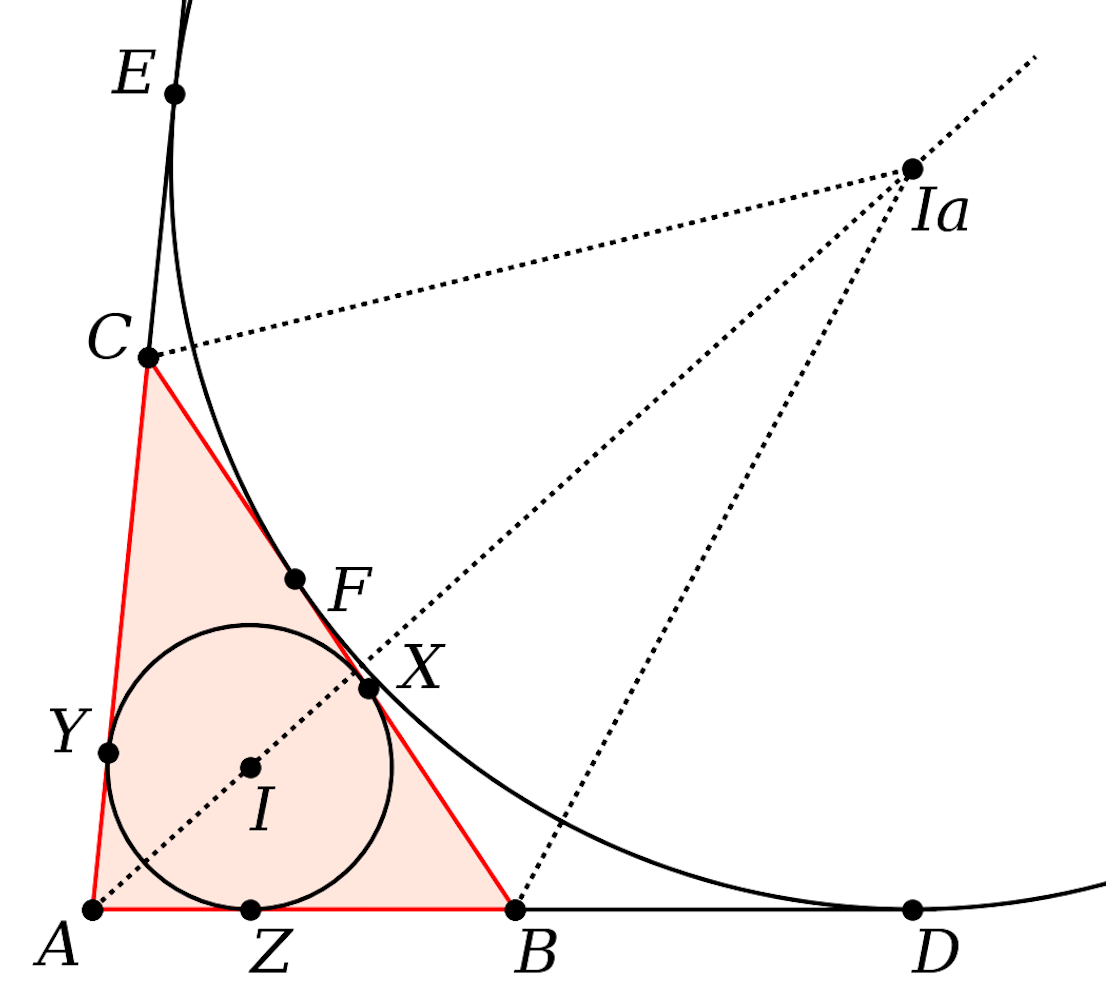
\includegraphics [scale=0.40] {excircle_crop1.png} \end{center}

Then let $s$ be half the perimeter, called the \emph{semiperimeter}:
\[ 2x + 2y + 2z = 2s \]
\[ x + y + z = s \]

so
\[ s = AZ + BX + CX \]
\[   = AZ + a \]
Re-arranging and generalizing 
\[ AZ = s-a \ \ \ \ \ \ \ \ BX = s-b \ \ \ \ \ \ \ \ CY = s-c \]
also
\[ s-a = (a+b+c)/2 - a \]
\[    = (-a+b+c)/2 \]
\[ 2(s-a) = -a+b+c \]

\subsection*{2}
Let 
$BD = BF = p$ and $CE = CF = q$.  We see that together $p + q = a$ so
\[ p = a - q \]

\begin{center} 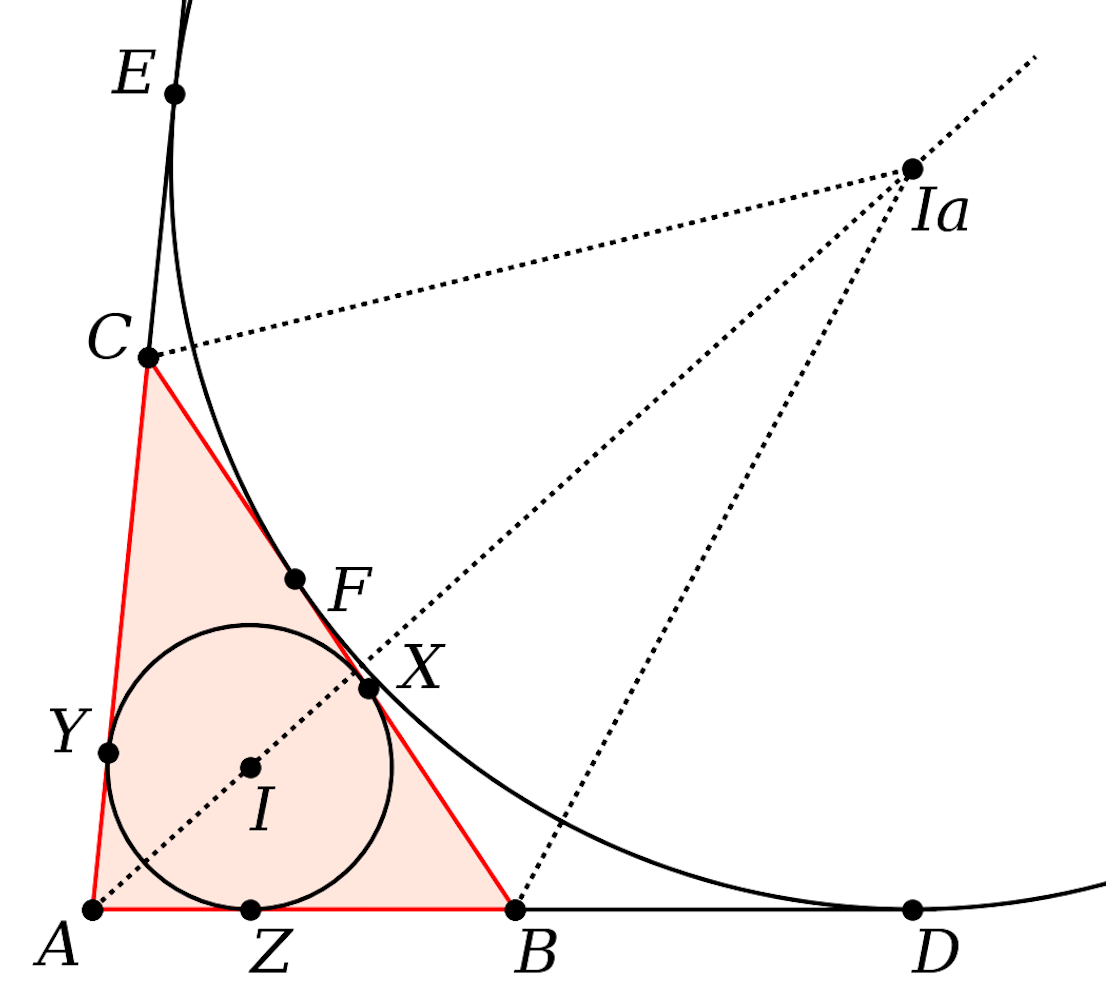
\includegraphics [scale=0.40] {excircle_crop1.png} \end{center}

The two tangents from $A$ to the excircle are also equal.  We have
\[ AD = AE \] 
\[ (s-a) + (s-b) + p = (s-a) + (s-c) + q \]
\[ p - b = q - c \]

Substituting
\[ a - q - b = q - c \]
\[ 2q = a - b + c \]
\[    = 2(s - b) \]
\[ q = s-b \]
Similarly
\[ p - b = a - p - c \]
\[ 2p = a + b - c = 2(s-c) \]
\[ p = s-c \]

Again, the two long tangents are equal:
\[ AD = s - a + s - b + s - c \]
\[ = 3s - 2s = s \]

\begin{center} 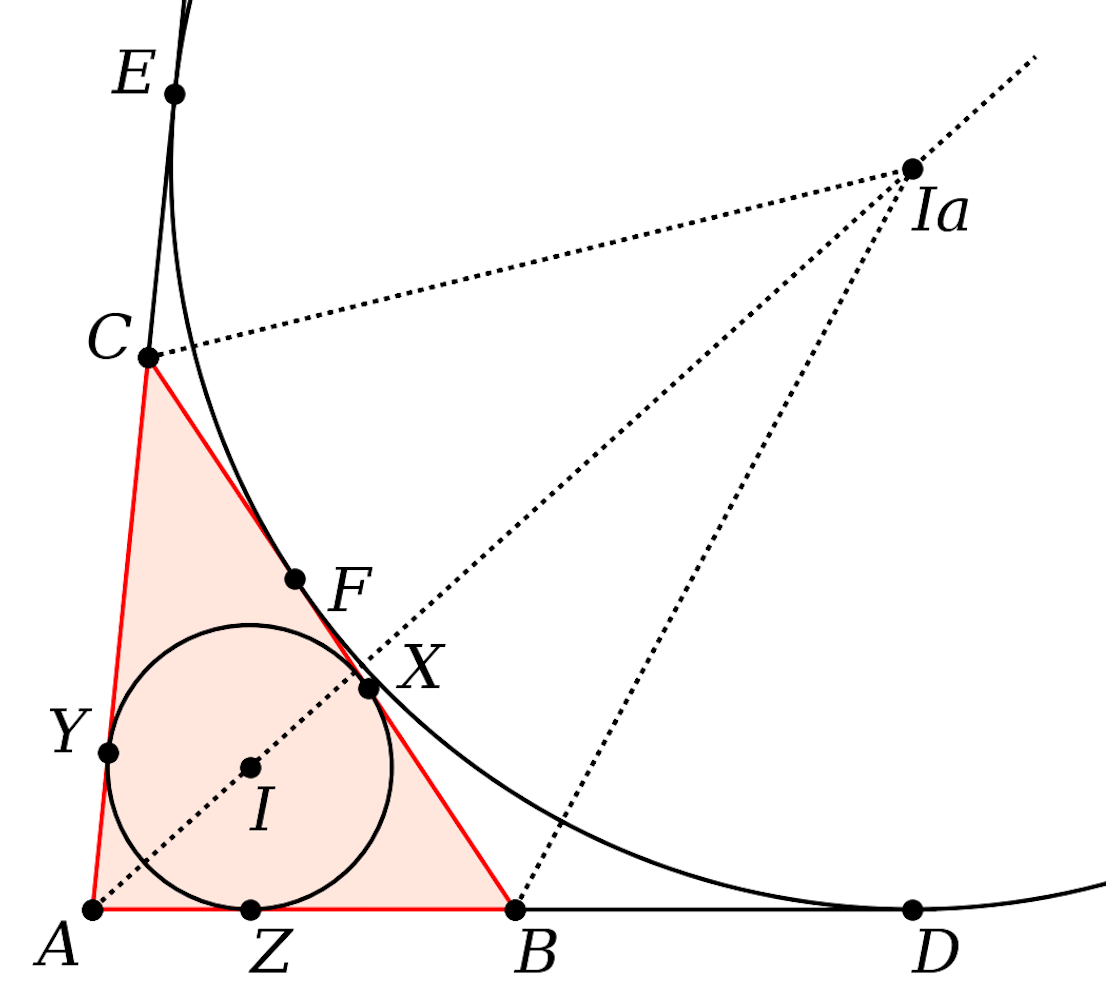
\includegraphics [scale=0.40] {excircle_crop1.png} \end{center}

The total length of the tangents $AD = AE$ is just $s$.

Also, the point $X$ divides the side $a$ into lengths $BX = s-b$ and $CX = s-c$.  Now we see that since (for example) $CE = CF = s-b$, the point $F$ (tangent to the excircle) divides the side $a$ into lengths $BF = s-c$ and $CF = s-b$.

\subsection*{3}

Comparing the incircle and excircle, we can find two similar right triangles:  $\triangle ADI_a$ and $\triangle AZI$.  The relevant ratios are
\[ \frac{R}{s} = \frac{r}{s-a} \]
\[ rs = R(s-a) \]
where $R = I_a D$ is the radius of the excircle on side $a$.

We have three pairs of congruent triangles so the total area of $\triangle ABC$ is
\[ \mathcal{A} =  rx + ry + rz = rs \]

\subsection*{4}

\begin{center} 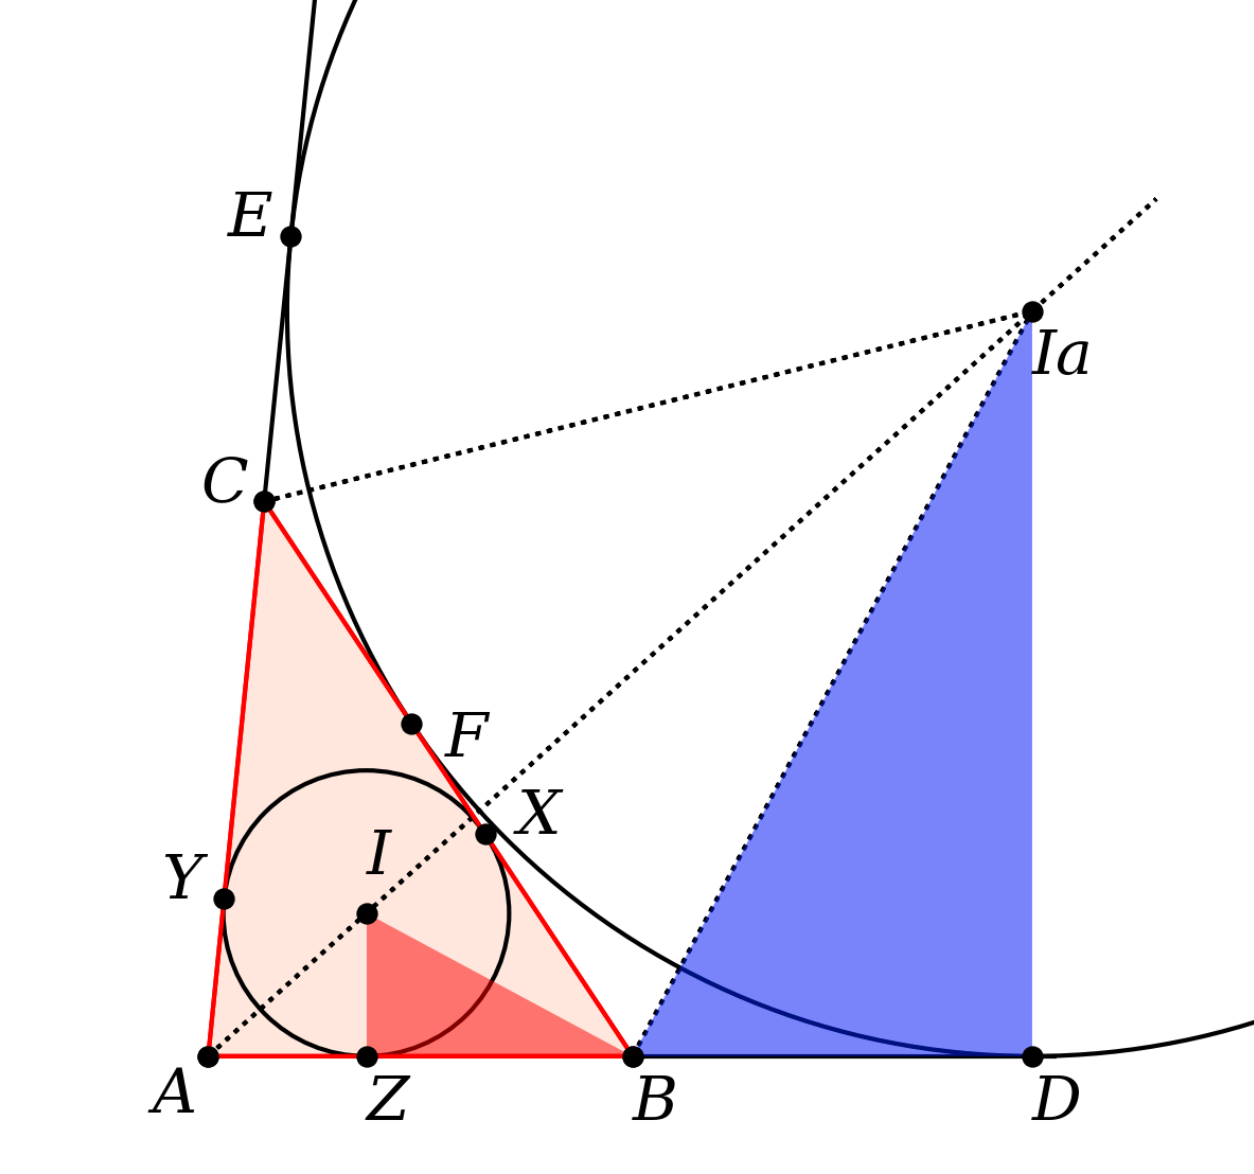
\includegraphics [scale=0.40] {excircle_crop2.png} \end{center}

It is a property of the internal and external angle bisectors that the sum of the half-angles is a right angle, since the internal and external angles are in total two right angles.  

So $\angle I B I_a$ is right.  It follows that $\angle IBZ$ and $\angle I_aBD$ are complementary.

Thus $\triangle IZB \sim \triangle BDI_a$ (marked red and blue in the figure).  The relevant ratios are:
\[ \frac{R}{s-c} = \frac{s-b}{r} \]
\[ Rr = (s-b)(s-c) \]

\subsection*{5}

We combine the last result from above with that from (3):
\[ rs = R(s-a) \]
Multiplying
\[ r^2Rs = R(s-a)(s-b)(s-c) \]
\[ r^2s = (s-a)(s-b)(s-c) \]
\[ r^2s^2 = s(s-a)(s-b)(s-c) \]

Since $rs = \mathcal{A}$ we have, finally
\[ \mathcal{A}^2 = s(s-a)(s-b)(s-c) \]

$\square$

This is Heron's theorem.  The square of the area of the triangle is equal to the product on the right.  As expected, the formula is symmetric in $a$, $b$ and $c$ and has the dimensions of the fourth power of a length.

\end{document}